\section{Proposed Method}
Figure~\ref{fig:process} illustrates the entire quantization flow for learned model compression which can be separated into three steps:

\begin{enumerate}
\item \textbf{Quantization Scheme Evaluation:} We define and analyze two quantization strategies in terms of their effectiveness for hardware-friendly execution their advantages and disadvantages during fine-tuning and the resulting performance.
\item \textbf{Layer-wise Precision Scaling:} To increase the model compression ratio we apply layer-wise precision scaling, meaning that for each layer different bit-widths are used for weights. Thereby we study the influence of selecting different bit-widths per layer on the resulting classification accuracy.
\item \textbf{Retraining with WQR and QR:} The last task focuses on reducing accuracy degradation occurring due to quantization. As loss of accuracy is induced due to the change of weight magnitudes when approximating them by rounding to the nearest quantization level, we aim to force weights to reduce their distance to such quantization levels in retraining, thus increasing classification accuracy of the quantized network.
\end{enumerate}

\begin{figure}[ht!]
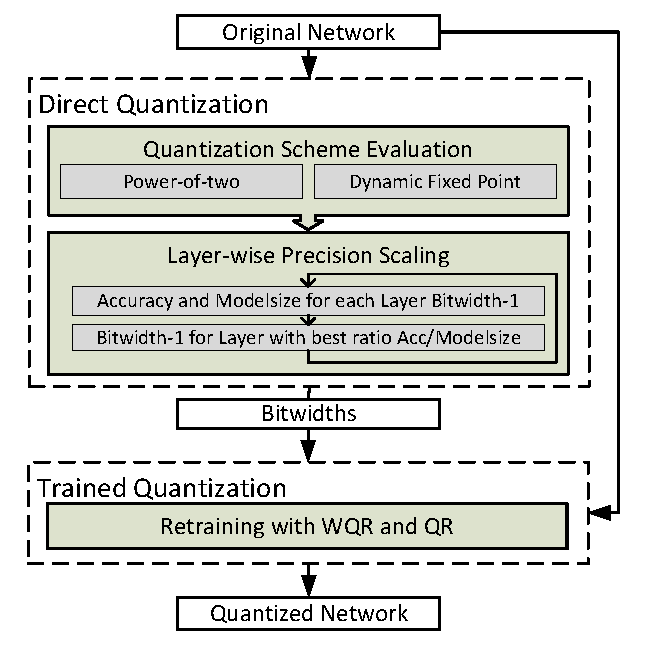
\includegraphics[width=\columnwidth]{img/process3.pdf}
\caption{Learned Weight Quantization step by step}\label{fig:process}
\end{figure}

While the first two steps serve for finding the best quantization method and 
bit-width for each layer when applying quantization without retraining, 
in the third step we perform retraining aiming to reduce the accuracy loss 
caused by quantization. In our flow, the weights are not first quantized and 
then retrained, but we always start from the high accuracy model, fine-tune 
weights with modified loss-functions and then perform quantization. This 
approach has the advantage that the network parameters are trained in full
precision but with the additional regularization terms which cause the weights 
to reduce their distance to the desired quantization levels before performing 
the actual quantization step. To better distinguish we use the term direct 
quantization for quantization without any fine-tuning. Trained quantization on the other hand consists of fine-tuning, followed by the actual quantization step. 
Input for the quantization process is a Deep Neural Network (DNN) $M$ with $N$ 
convolutional and/or fully connected layers and weight-tensors $W_n, 0<n<N$ of 
arbitrary resolution. Details on the network used for evaluation can be found in 
table \ref{tab:allconv}. Table \ref{tab:variables} summarizes the list of 
variables used in this work.

\begin{table}[ht!]
  \caption{Variables used in this work}
  \label{tab:variables}
  \begin{tabular}{ccl}
    \toprule
    	\textbf{Variable}&\textbf{Comment}\\
    \midrule
 		$M$& Original network model\\
		$M_q$ & Quantized network model\\
 		$N$& Number of layers\\
		$W_n$ & Original Weights\\
		$W_{q_n}$ & Quantized weights\\
		$b_n$ & Bit-widths for layers $n = 0...N$\\
		$Q_n$ & Quantization schemes for layers $n = 0...N$\\
		$Q_{p2}$ & Power-of-2 quantization scheme\\
		$n_1$ & Maximum exponent for Power-of-2 quantization\\
		$n_2$ & Minimum exponent for Power-of-2 quantization\\
		$s$ & Maximum absolute weight within the selected layer\\
		$Q_{dfp}$ & Dynamic Fixed Point quantization scheme\\
		$B$ & Unscaled Dynamic Fixed Point quantization scheme\\
		$acc_M $ & Classification accuracy of the original network\\
		$acc_{M_q} $ & Classification accuracy of the quantized network\\
		$\Delta acc $ & Accuracy degradation due to quantization\\
		$W_{mem} $ & Weight memory bits\\
		$\lambda_1 $ & Quantization-Regularization scale factor\\
		$QR $ & Quantization-Regularization Term\\
		$\lambda_2 $ & Weighted Quantization-Regularization scale factor\\
		$WQR $ & Weighted Quantization-Regularization term\\
  \bottomrule
\end{tabular}
\end{table}

%Aiming at hardware friendly implementation, in contrast to other works (e.g. \cite{Zhou2017a}) we absorb Batch-Normalization layers into the convolutional layers weights and biases, as they induce additional computational complexity and increase model size \cite{Ioffe2015}. This absorption can be performed without any performance degradation or retraining as Batch-Normalization merely presents a linear transformation to the input or output map of the preceding respectively succeeding layer. \todo[inline]{maybe add effect on number of computations and model size}

\subsection{Direct Quantization}
\label{subsec:quant}
In direct quantization, the original network $M$ is expressed as $M_q$ where 
the weights $W_n$ of each layer are represented as $W_{q_n}$. The values of 
$W_{q_n}$ are determined by rounding each element of $W_n$ to the quantization 
level with the smallest absolute distance of a previously defined quantization 
scheme $Q$.

\subsubsection{Quantization Scheme Evaluation}
Here, we present Power-of-two \cite{Zhou2017a} and Dynamic Fixed Point 
\cite{Hubara2016, Gysel2016a}, two different quantization schemes and 
compare their properties for direct and trained quantization.

\paragraph{Power-of-two quantization}
We implement Power-of-two (Po2) quantization similar as in \cite{Zhou2017a}. $Q_{p2}$ is given as
\begin{equation}\label{eq:pow2_quant}
Q_{p2} = \{\pm 2^{n_1},... ,\pm 2^{n_2},0\}.
\end{equation}
$n_1$ and $n_2$ are integers with
\begin{eqnarray}
n_1 &=& \lfloor log_2 \frac{4s}{3} \rfloor \label{eq:n1_max}\\
s &=&  max(abs(W)). \label{eq:s_max}
\end{eqnarray}
For a given bit-width $b$ and $n_2$ are defined by
\begin{equation}\label{eq:n2}
n_2 =  n_1 - (2^{b-1} -1).
\end{equation}

Thus, the quantization levels depend on the distribution of weights, 
especially on the weight with the highest absolute value. By adding `$0$' as 
a quantization level, we enable power-of-two quantization to also serve as a 
pruning mechanism when applied to weight matrices, as small weights are rounded 
to zero. In experiments symmetrical quantization schemes lead to higher 
classification accuracies for the quantized networks, 
therefore we only use $2^b-1$ of $2^b$ possible quantization levels.
%\cite{Zhou2017a}

\paragraph{Dynamic Fixed Point}
Dynamic fixed point (DFP) data type is successfully used in several works for either direct quantization or retrained model compression \cite{Hubara2016, Gysel2016a}.
For DFP quantization, we first define a set of $2^{b}-1$ equidistant quantization levels:
\begin{equation}\label{eq:dfp_nums}
B = \{\pm 2^{b-1}-1,\pm 2^{b-1}-2,... ,0\}.
\end{equation}
Similarly to Po2 quantization, we prefer a symmetric quantization scheme. 
Next $B$ is normalized and scaled, depending on the distribution of weights:
\begin{equation}\label{eq:dfp_quant}
Q_{dfp} = \frac{B}{2^{b-1}}*2^{n_1}.
\end{equation}

Figure \ref{fig:quant_hist} depicts the distribution of weights for an 
example layer of a CNN, before and after quantization. While 
figure \ref{fig:quant_hist}(a) shows the distribution for Po2 quantization, 
figure \ref{fig:quant_hist}(b) illustrates the distribution for DFP quantization. 
As can be seen that po2 has much irregular quantization values compared to DFP, 
and also considers the values close to `0' which might help to retain the 
information with lower weights and aid in improving the accuracy.


\begin{figure}[ht!]
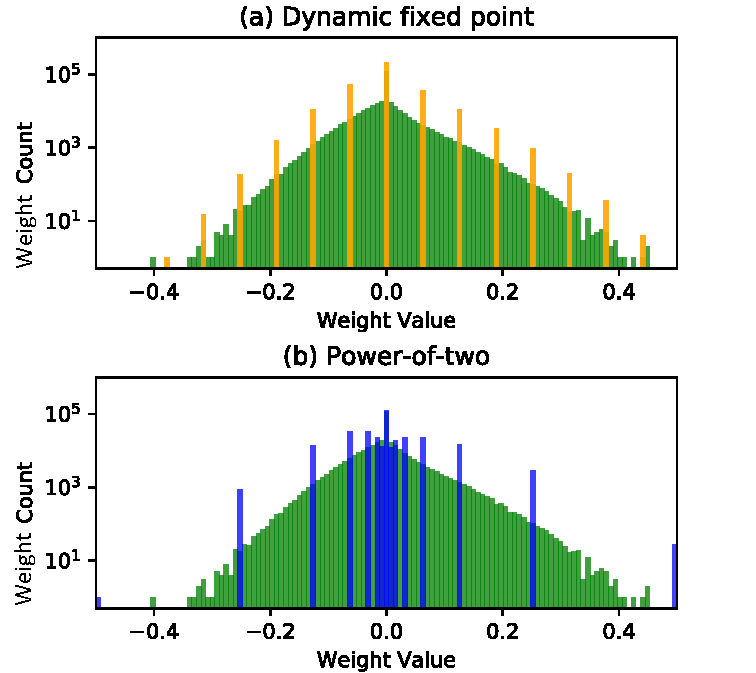
\includegraphics[width=\columnwidth]{img/histograms2.pdf}
\caption{Distributions before and after direct weight quantization for (a) Dynamic Fixed Point and (b) Power-of-two quantization}\label{fig:quant_hist}
\end{figure}

As accuracy degradation of the quantized model $M_q$ in comparison to the original model $M$ is a result of the quantization error, it is necessary to understand the relation between bit-width and quantization error for both datatypes.

With DFP quantization, the mean square error (MSE) can be reduced with 
increasing bit-width, since every additional bit divides the intervals in 
half (see fig. \ref{fig:quant_hist}a). 
Meanwhile when increasing bit-width in Po2 quantization, the new quantization levels are always added close to `0' (see fig. \ref{fig:quant_hist}b). As a consequence with Po2 quantization, the quantization error can only be reduced to a certain extent. Figure \ref{fig:quant_mse} shows the resulting mean square errors for one weight-tensor of an example layer when applying different bit-widths.

\begin{figure}[t]
%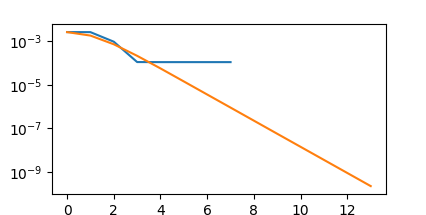
\includegraphics[width=\columnwidth]{img/MSE.PNG}
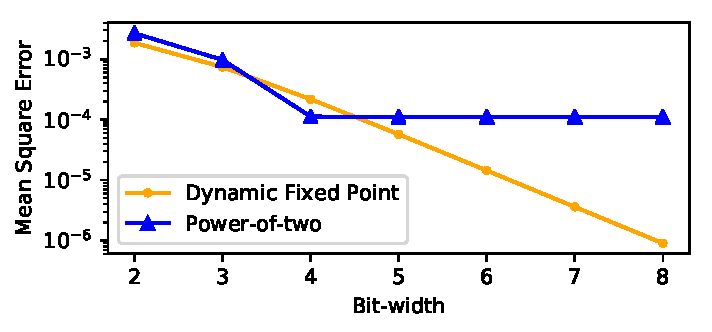
\includegraphics[width=\columnwidth]{img/mse.pdf}
\caption{Mean square error for an example layer when applying Power-of-two and Dynamic Fixed Point quantization with different bit-widths. While when using DFP quantization the error decreases exponentially, for Po2 quantization the quantization error reaches the minimum already at bit-width 4}\label{fig:quant_mse}
\end{figure}

In addition, we consider the amount of pruned weights as an important factor for model compression. In comparison to DFP, Po2 quantization decreases sparsity within the weight matrices as a result of quantization, due to the higher density of levels close to `0'. Therefore to fully benefit from the advantages of sparsity, an additional pruning step before retraining is recommended. In figure \ref{fig:quant_sparse} the number of pruned weights depending on the selected bit-width is shown for Po2 and DPF quantization.

\begin{figure}[t]
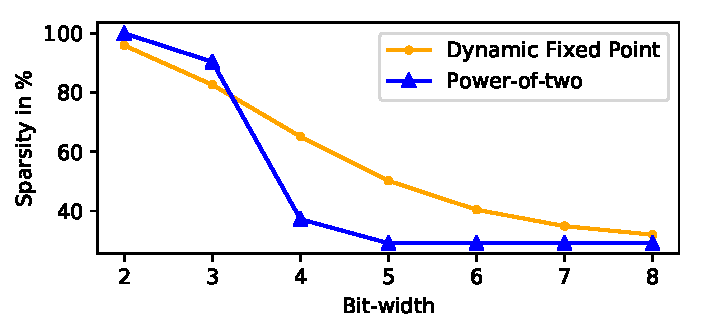
\includegraphics[width=\columnwidth]{img/sparse.pdf}
\caption{With increasing bit-widths the sparsity due to quantization decreases for Dynamic Fixed Point and Power-of-two quantization. Sparsity is denotes the amount of weights that are 0 relative to the total amount of Weights}\label{fig:quant_sparse}
\end{figure}

%AJ: I reformulated the following paragraph to make it clearer:
Figures \ref{fig:quant_mse} and \ref{fig:quant_sparse} suggest that for direct Po2 quantization bit-widths higher than 4-bit do not further decrease the $\Delta acc$ but 4-bits in comparison to 5-bits slightly increase sparsity. 
%Figures \ref{fig:quant_mse} and \ref{fig:quant_sparse} suggest that for direct Po2 quantization bit-widths higher than 4-bit cannot further decrease the resulting $\Delta acc$. Furthermore, since 4-bit Po2 in comparison to 5-bit Po2 increases sparsity, but does not significantly increase the MSE, we can suspect similar results in terms of accuracy but more pruned weights for 4-bit Po2. 
On the other hand, by scaling the bit-width of DFP the resulting MSE can be reduced exponentially (Fig. \ref{fig:quant_mse}) meaning that even bit-widths higher than 8 bit deliver more accurate results. In terms of sparsity, DFP prunes more weights than Po2 for bit-widths of four and higher.

Based on these observations we expect that for direct DFP quantization $\Delta acc$ can be reduced to almost 0, based on Layer-wise Precision Scaling. For direct Po2 quantization we expect a higher $\Delta acc$ and no significant increase of accuracy for bit-widths higher than five. It can be seen in figures \ref{fig:lw_scale} and \ref{fig:lw_100} that these expectations are confirmed.
%\caj{Are these expectations confirmed? If yes, let's point to the graph or section, where this is evident.}

\subsubsection{Layer-wise Precision Scaling}
\label{layerwise}
Secondly, to further reduce the model-size, we apply different quantization schemes per layer by optimizing bit-widths. In comparison to choosing equal bit-width for each layer, due to the varying amount of parameters and varying distribution of weights between layers, selecting fitting quantization schemes for each layer can enable lower bit-widths per layer without reducing the resulting accuracy.  For the experiments we assume either DFP or Po2 quantization. For an arbitrary network $M$ with accuracy $acc_{M}$ applying weight quantization with the set of bit-widths $b_n$ leads to accuracy $acc_{Mq}$
and weight memory bits\highlight{
\begin{equation}\label{eq:w_mem}
W_{\text{mem}} = \sum^N_n{\text{card}(W_n)*b_n}
\end{equation}
where $\text{card}(A)$ denotes the cardinality of set $A$.}
%AJ: Symbols with more than one letter are better typeset as\text{} in math mode.
For each $b_n$ we compute the resulting accuracy degradation
\begin{equation}\label{eq:acc_deg}
\Delta acc = acc_{M} - acc_{Mq}
\end{equation}
and iteratively decrease the bit-width of the layer where a lower bit-width leads to the smallest product of $\Delta acc * W_{mem}$  (see algorithm~\ref{alg:lw}).

\begin{algorithm}
\caption{Layer-wise Precision Scaling}\label{alg:lw}
\begin{algorithmic}
\State 
\Procedure {Layer-wise Precision Scaling}{$M$}
	\State initialize $b_n$
	\While{$\Delta acc < \epsilon$}
		\ForAll{$n$ in layers}	
			\State bitwidth of $layer_n$ - 1
			\State Compute $Acc_{M_q}$, $\Delta acc$ and $W_{mem}$
			\State bitwidth of $layer_n$ + 1
		\EndFor	
		\State Decrease bitwidth of layer with smallest $\Delta acc * W_{mem}$
	\EndWhile
\EndProcedure
\end{algorithmic}
\end{algorithm}
Figure \ref{fig:lw_scale} shows the results for Layer-wise Precision Scaling performed by algorithm \ref{alg:lw} on All-Convolutional Network \cite{Springenberg2015} for CIFAR-10. We can deduce that while DFP quantization also allows direct quantization, whereas for power-of-two quantization almost always an additional fine-tuning step is necessary to achieve high accuracy results.

\begin{figure}[t]
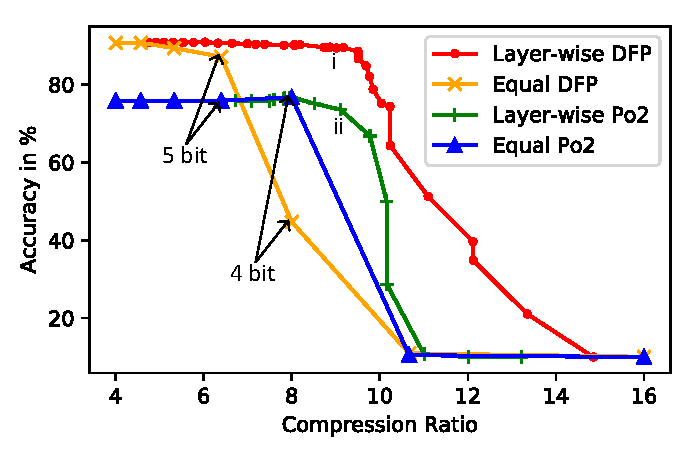
\includegraphics[width=\columnwidth]{img/layerwise.pdf}
\caption{Layer-wise Precision Scaling compared with equal bit-width quantization for DFP and Po2 quantization. Compression ratio is the ratio between 32bit weight memory and the weight memory for the quantized network. Point i indicates DFP with $b_n=\lbrack$7 7 7 4 4 3 3 7 7$\rbrack$ , point ii indicates Po2 with $b_n=\lbrack$4 4 4 4 3 3 4 4 4$\rbrack$.}\label{fig:lw_scale}
\end{figure}

\subsection{Trained Quantization}
The used datasets (CIFAR-10, CIFAR-100 and SVHN) are already divided into \textbf{test data} and \textbf{training data}. While with Layer-wise Precision Scaling as described in section \ref{layerwise} focuses on decreasing $\Delta acc * W_{mem}$ without retraining, we can additionally reduce $\Delta acc$ by retraining the original network on the training data with the goal of increasing accuracy of the classifier on test data. As a consequence we use the performance metrics in table \ref{tab:metrics}.
\begin{table}[ht!]
  \caption{Performance Metrics used for Fine-tuning}
  \label{tab:metrics}
  \begin{tabular}{ccc}
    \toprule
    	\textbf{Variable}&\textbf{Metrics}&\textbf{Comment}\\
    \midrule
 		$acc_{tr}$&Training Accuracy& Accuracy of the network\\
 		&&  on the training data\\
		$acc_M$&Test Accuracy & Accuracy of the  network \\
 		&&  on the test data\\
		$acc_{M_q}$&Quantized & Accuracy of the network \\
		&Test Accuracy\footnotemark& with quantized weights\\
		&& on the test data\\
		$acc_{init}$&Init. Quantized & Accuracy of the network \\
		&Test Accuracy& with direct quantized initial\\
		&&weights on the test data\\
		CR& Compression Ratio & Ratio $W_{Mem}$ of original model\\
		& & to $W_{Mem}$ of quantized model\\
  	\bottomrule
\end{tabular}
\end{table}
\footnotetext{For the computation of Quantized Test Accuracy, the weights of the network are directly quantized after each epoch.}

\subsubsection{Quantization-Regularization}
\label{subsec:qr}
To decrease $\Delta acc$ for a selected set of bit-widths $b_n$, we need to find the best set of $W_n$ so that approximation with $Wq_n$ achieves a maximum of $acc_{Mq}$. As shown in \cite{Lin2015a, Shin2017} the degradation of classification accuracy of a DNN due to quantization is directly related to the signal to quantization-noise ratio (SQNR) and the amount of weights per layer, as both influence the SQNR of the intermediate layer outputs and as a consequence the resulting network outputs. Therefore retraining network weights to achieve lower SQNR without reducing $acc_{M}$, leads to an increased accuracy of the quantized network.
To enforce weight quantization during the training phase we define the quantization-regularization (QR) term as\highlight{
\begin{equation}\label{eq:quant_reg}
QR = \sum^{N}_{n}\sum^{\text{card}(W_n)}_{i}\frac{\mid W_{n_i}-Wq_{n_i}\mid}{\max(Q_n)*\text{card}(W_n)}
\end{equation}
 }
which expresses the mean of the absolute weight distances of each weight to the corresponding quantized value.

By adding the QR-term to the loss function (eq. \ref{eq:lossfunction}) weights are forced closer to the quantization levels during retraining.
\begin{equation}\label{eq:lossfunction}
\textrm{Modified Loss = Loss}+\lambda_1*QR
\end{equation}
During fine-tuning with the parameter $\lambda_1$ the trade-off between $min(Loss)$ and $min(QR)$ and, as a consequence, between $min(\Delta accuracy)$ and $max(acc_{M})$ can be adjusted. For the experiments we applied fixed $\lambda_1$ and linearly increasing $\lambda_1$ (e.g. $\lambda_1=10*epoch$). Figure \ref{fig:weightreg} depicts the trained quantization process. With each epoch the weights are pulled closer to the quantization levels, thus decreasing $QR$ and $\Delta acc$.

\begin{figure}[ht!]
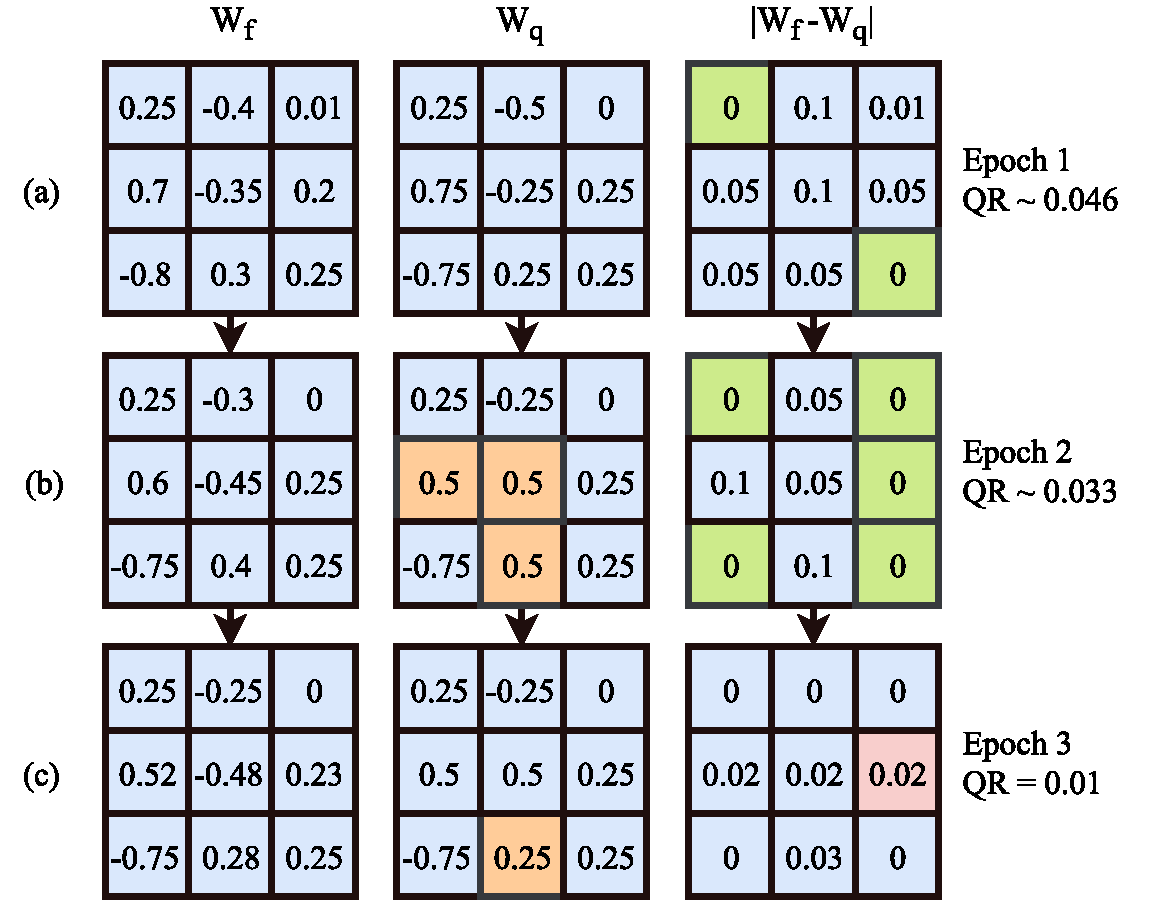
\includegraphics[width=\columnwidth]{img/weightreg.pdf}
\caption{Illustration of Quantization-Regularization. The first column shows the floating point values of the weights on which the actual training is performed. The second column shows the quantized weights, and the third column the element-wise absolute difference of floating point and quantized weights. Changes of quantized weights are marked in the second column. \highlight{Weight update for $W_f$ is performed based on backpropagation of the modified loss function (eq. \ref{eq:lossfunction}).} Successfully quantized weights are marked in the third column. After Epoch 1 (a) the weights are hardly regularized and $QR$ is relatively large. Epoch 2 (b) shows that due to regularization, weights are pulled closer to the quantization levels $\mathbf{Q_n=\{0,\pm 0.25, \pm 0.5, \pm 0.75\}}$ and $QR$ gets smaller. For three of the weights the resulting quantization level changed, and weights decrease their distance to the next quantization level. Epoch 3 (c) shows further reduction of the $QR$ term.}\label{fig:weightreg}
\end{figure}

While choosing a high ($>1000$) $\lambda_1$ leads to fast quantization with strong accuracy degradation, a low $\lambda_1$ value ($<1$) does not enforce quantization. Either way, much like weight decay low $\lambda_1$ values can help avoiding overfitting during training.

\subsubsection{Weighted Quantization-Regularization}
\label{subsec:wqr}
While in normal QR each weight within one layer is considered equally important for reaching high classification accuracy, the efficiency of pruning \cite{Han2015a,Yang2017,Dong2017} shows that especially weights with small magnitudes can be changed without reducing the accuracy of the network.
Similarly to \cite{Zhang2015}, the weights can be divided into two disjoint subsets, where QR is applied on one of the subsets while the other weights are being retrained without QR. Going one step further we can multiply the QR value of each weight with the absolute magnitude of the weight.
\footnote{Previously the sum of weights is normalized to 1 for each layer}
This strategy forces quantization stronger on weights with higher magnitudes which can be especially useful for Po2 quantization, where density of quantization levels decreases with increasing weight values. Therefore we define the Weighted Quantization-Regularization (WQR) term as\highlight{
\begin{equation}\label{eq:w_quant_reg}
WQR = \sum^{N}_{n}\sum^{\text{card}(W_n)}_{i}(\frac{\mid W_{n_i}-Wq_{n_i}\mid\mid W_{n_i}\mid}{\max(Q_n)^2*\text{card}(W_n)}
\end{equation}}
and similarly to equation \ref{eq:lossfunction} we can weight the trade-off between accuracy and weight regularization with $\lambda _1$ and $\lambda _2$ (eq. \ref{eq:lossfunction2})

\begin{equation}\label{eq:lossfunction2}
\textrm{Modified Loss = Loss} + \lambda _1 *QR + \lambda _2 *WQR
\end{equation}

Again during training the parameters $\lambda_1$ and $\lambda_2$ have to be adjusted carefully to reach the desired improvement of $Acc_{Mq}$, without at the same time decreasing $Acc_{M}$. In our experiments we found a linear increasing $\lambda_2$ to work best (e.g. $\lambda_2 = 10*\textrm{epoch}$).

For fine-tuning, we use algorithm \ref{alg:quant}.

\begin{algorithm}[ht!]
\caption{Fine-tuning with Quantization-Regularization and Weighted Quantization Regularization}\label{alg:quant}
\begin{algorithmic}
\State 

\Procedure {Trained Quantization}{$M$, $b_n$, $\lambda_1$, $\lambda_2$}
	\For{epochs}
		\ForAll{Mini Batches} \Comment{Train on Training Data}
			\For{$n >= N$}	\Comment{Quantize all Layers}
				\State $Q_n(W_n,b_n)$ \Comment{Determine Quantization Scheme}	
				\State $W_{q_n}$ = Quantize($W_n$,$Q_n$) \Comment{Quantize Weights}		
			\EndFor
			\State Loss + $\lambda_1*QR(W_n, Q_n, W_{q_n}) + \lambda_"*WQR(W_n, Q_n, W_{q_n})$
			\State Backpropagation(Loss,QR,WQR,$\lambda_1$,$\lambda_1$)		
		\EndFor	
		\State Compute $Acc_{M}$	\Comment{Test Accuracy}
		\State Compute $Acc_{M_q}$	\Comment{Quantized Test Accuracy}
	\EndFor
	\State \textbf{return} $M_q$	\Comment{Return Quantized Model}
\EndProcedure
\end{algorithmic}
\end{algorithm}


Figure \ref{fig:acc_example} illustrates the fine-tuning process for 4-bit equal bit-width Po2 quantized All-Convolutional Net for CIFAR-10. At the beginning of the fine-tuning process the term $\lambda_2*WQR$ increases due to the increasing $\lambda_2$ value, while the $WQR$-Term decreases exponentially. At Epoch 200 learning rate is decreased from $1e^{-4}$ to $1e^{-5}$ leading to the drop of $\lambda_2*WQR$. This can be explained by fact that a larger learning rate leads to larger weight changes. If the weights are already close to the quantization levels a lower learning rate can lead to better approximation of the weights to the quantization levels.
\begin{figure}[ht!]
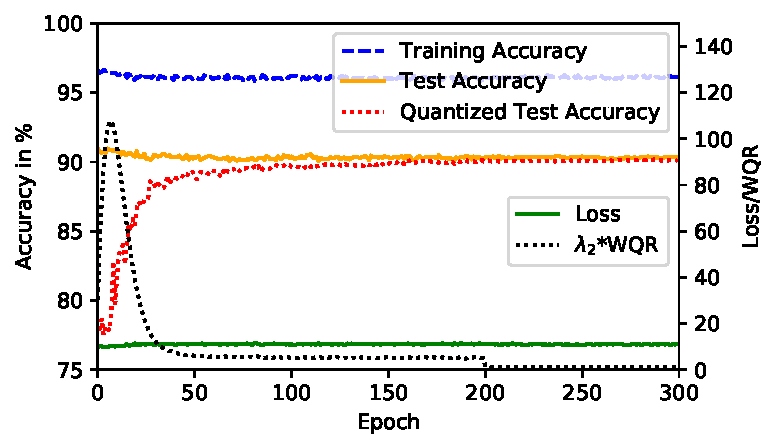
\includegraphics[width=\columnwidth]{img/accuracy.pdf}
\caption{Fine-tuning of All-Convolutional Net for CIFAR-10 with linear increasing $\pmb{\lambda}\mathbf{_2}$ for 4-bit equal bit-width Po2 quantization. $\pmb{\Delta}\mathbf{Acc}$ is decreased from $\mathbf{14.09\%}$ to $\mathbf{0.14\%}$ resulting in Quantized Test Accuracy of $\mathbf{90.18\%}$ in comparison to initial Floating Point Test Accuracy $\mathbf{90.83\%}$.}
\label{fig:acc_example}
\end{figure}




%Adaptive methods give a good idea of how models can be approximated by simply transforming them, but when retraining the question is how to choose the best bitwidth per layer. We can use quantization-regularization and observe how the weights get closer to the quantization levels. If the MSE stays big for one layer, that basically means, that the bitwidth for that layer should be approximated with a higher precision.


\subsection{Summary and Analysis}
In combination, the discussed techniques for quantization (sec.~\ref{subsec:quant}), Layer-wise Precision Scaling (sec.~\ref{layerwise}) and fine-tuning with QR (sec.~\ref{subsec:qr}) and WQR (sec.~\ref{subsec:wqr}) facilitate DNN weight compression.

The above discussed two quantization schemes behave differently during the quantization process and require different quantization strategies. For bit-widths higher than 7 bit DFP can be applied without any retraining and still achieves almost floating point accuracy. For equal bit-width DFP quantization with 7 bit and less, $\Delta acc$ increases and fine-tuning is necessary to reach the accuracy of the original network. On the other hand Po2 quantization always requires retraining, as even the use of bit-widths higher than five reduce the quantization error only to a certain extent.

To increase the compression ratio when applying DFP quantization, layer-wise precision scaling is an effective method, since not all layers require the same the bit-width for high accuracy. For instance, in modern convolution-only networks, layers with fewer parameters require larger bit-widths~\cite{Lin2015a}. As a result, when applying layer-wise precision scaling the weights of the output and input layers are kept at high precision, as they usually have the fewest parameters.
In comparison to DFP, for Po2 quantization, layer-wise precision scaling does not proof to be as effective, as almost the same bit-width is recommended throughout the network to achieve best accuracy.

\begin{figure}[ht!]
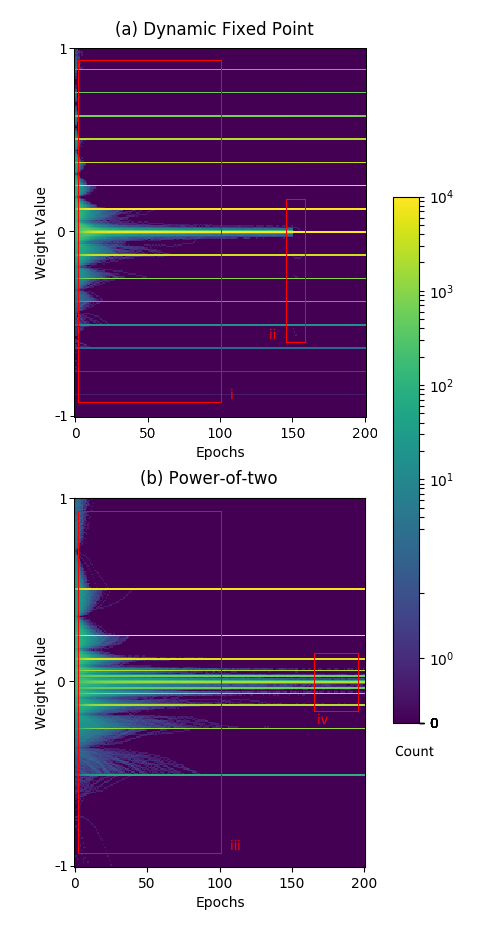
\includegraphics[width=\columnwidth]{img/histotime2.png}
\caption{Distribution of weights in layer 5 of AllConvNet (CIFAR-10) during fine-tuning with WQR and QR to (a) 4-bit Dynamic Fixed Point and (b) 4-bit Po2. DFP (a) is trained with $\mathbf{\lambda_2 = epoch*10}$. Region i shows the faster quantization of weights with high magnitudes and slower quantization of weights close to 0. At epoch 150 QR is applied with $\mathbf{\lambda_1 = 100}$ to quantize also weights with smaller values (ii). Po2 (b) is trained with $\mathbf{\lambda_2 = epoch*10}$. Region iii also shows slower quantization for small magnitude weights. Due to the distribution of quantization levels, weights around 0 are already close to the next quantization level (iv).}
\label{fig:WQR_QR}
\end{figure}

For fine-tuning of Po2 and DFP quantized networks, QR and WQR can be added to the loss function as regularization terms to force quantization during retraining. While the QR term forces all weights equally to reduce the distance to the next quantization level, the WQR term is reduced for weights with small magnitudes. Therefore, WQR operates less restrictive than QR, as the original QR value is multiplied with a factor from 0 to 1 (normalized weight magnitude). As a consequence it is an effective strategy to apply WQR followed by QR fine-tuning.

Figure \ref{fig:WQR_QR} shows the distribution of weights in layer 5 during (a) 4-bit DFP and (b) 4-bit Po2 quantization of the All-Convolutional Network for the CIFAR-10 dataset. For fine-tuning to 4-bit DFP quantization (Fig.\ref{fig:WQR_QR}a) $\lambda_2$ is increased linearly by a factor of 10 with each epoch. As QR scale factor $\lambda_1$ we use 0 before and 100 starting at epoch 150. Region i in figure \ref{fig:WQR_QR}a shows the decelerated quantization of small magnitude weights. Starting with epoch 150, also weights close to 0 are quantized, due to the application of QR (Fig. \ref{fig:WQR_QR}a,ii). For 4-bit Po2 quantization only WQR is necessary ($\lambda_2 = epoch*10$) to achieve quantization. Due to the the non-equidistant distribution of quantization levels in Po2 quantization, the weights with high magnitudes take longer than in DFP quantization to reach the quantization levels (Fig. \ref{fig:WQR_QR}b,iii). Additional QR is not necessary since, due to the high density of quantization levels close to 0, the weights with smaller magnitudes induce a very small quantization error (Fig. \ref{fig:WQR_QR}b,iv).

QR and WQR enable trained quantization to improve performance in comparison to direct quantization. Regularization-based quantization is very simple to implement and applicable for any quantization scheme. As a consequence QR and WQR could be employed alongside other effective quantization techniques such as stochastic quantization. Besides the simplicity of the approach, it also allows a deeper analysis of quantization schemes by recording the change of weight distribution during training.

While enabling compression for more efficient inference, during training QR and WQR add overhead due to the mandatory quantization step after each mini-batch and the necessary computations for calculation of QR and WQR. The fact that all weights have to be stored as floating point values and quantized values, increases the weight memory during training by a factor of 2.

%Since the number of weights in state-of-the-art DNNs is smaller by at least the factor 100 than the MACs required for one feed forward computation, we can neglect this disadvantage. 

